\section{Базы данных  и выравнивание}

\begin{frame}{UniProt Knowledgebase}
    UniProtKB – две базы аннотированных белковых последовательностей с общим форматом
записей.
\begin{itemize}
    \item \textbf{TrEMBL} (от Translated EMBL) – автоматическая база данных, содержащая, в основном,
формальные трансляции открытых рамок считывания, предсказанных в нуклеотидных последовательностях.
    \item \textbf{Swiss-Prot} (раньше была отдельным банком) – курируемая база данных. Кураторы выбирают
записи из TrEMBL, проверяют и дополняют их, переносят в Swiss-Prot.
\end{itemize}
\end{frame}

\begin{frame}{Рост числа записей в Swiss-Prot}
    \centering
    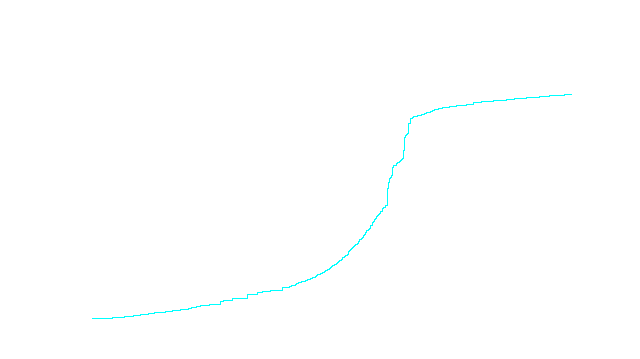
\includegraphics[height=0.9\textheight]{uniprot-stat1}
\end{frame}

\begin{frame}{Одна запись UniProtKB}
    \begin{itemize}
        \item     Одна запись – все продукты одного гена из организмов одного вида. Известные изоформы,
полиморфизмы и т.д. указывают в аннотации записей.
        \item Изоформы указаны в полях СС (подраздел "Alternative products") и FT (конкретные участки
различий), полиморфизмы указывают в поле FT.
    \item Правило не строгое, из него есть исключения. Например, если для гена известно множество
изоформ, сильно отличающихся по последовательности и функциям, то для них создадут несколько записей
    \end{itemize}
\end{frame}

\begin{frame}[fragile]{Таблица локальных особенностей (Feature table, FT)}
Имеет строгий формат, список и описание всех возможных ключей доступно на сайте UniProt.
\begin{multicols}{2}
    \tiny
    \begin{verbatim}
FT CHAIN 1..188
FT /note="Isochorismatase family protein YecD"
FT /id="PRO_0000201831"
FT HELIX 6..8
FT /evidence="ECO:0000244|PDB:1J2R"
FT STRAND 9..14
FT /evidence="ECO:0000244|PDB:1J2R"
FT REGION 5..34
FT /note="Interaction with RNase E"
FT ACT_SITE 209
FT /note="Proton donor"
FT /evidence="ECO:0000255|HAMAP-Rule:MF_00318,
FT ECO:0000269|PubMed:15003462"
FT METAL 246
FT /note="Magnesium"
FT /evidence="ECO:0000269|PubMed:11676541,
FT ECO:0000269|PubMed:16516921"
FT BINDING 159
FT /note="Substrate"
FT /evidence="ECO:0000255|HAMAP-Rule:MF_00318"
FT MOD_RES 257
FT /note="N6-acetyllysine"
FT /evidence="ECO:0000269|PubMed:18723842"
FT CONFLICT 180..188
FT /note="SVEEILNAL -> TWKRSSTRYDLHRSTAMVAS (in Ref. 1)"
\end{verbatim}
    \columnbreak
    \normalsize
    вторичная структура\\
    \vspace{1cm}
сайты связывания\\
    \vspace{1cm}
модифицированные остатки\\
    \vspace{1cm}
разночтения в
последовательности\\
    \vspace{1cm}
и т.д.
\end{multicols}
%\begin{tikzpicture}
%    \node (A) {}
%\end{tikzpicture}
\end{frame}

\begin{frame}{Выравнивание}
    \centering
    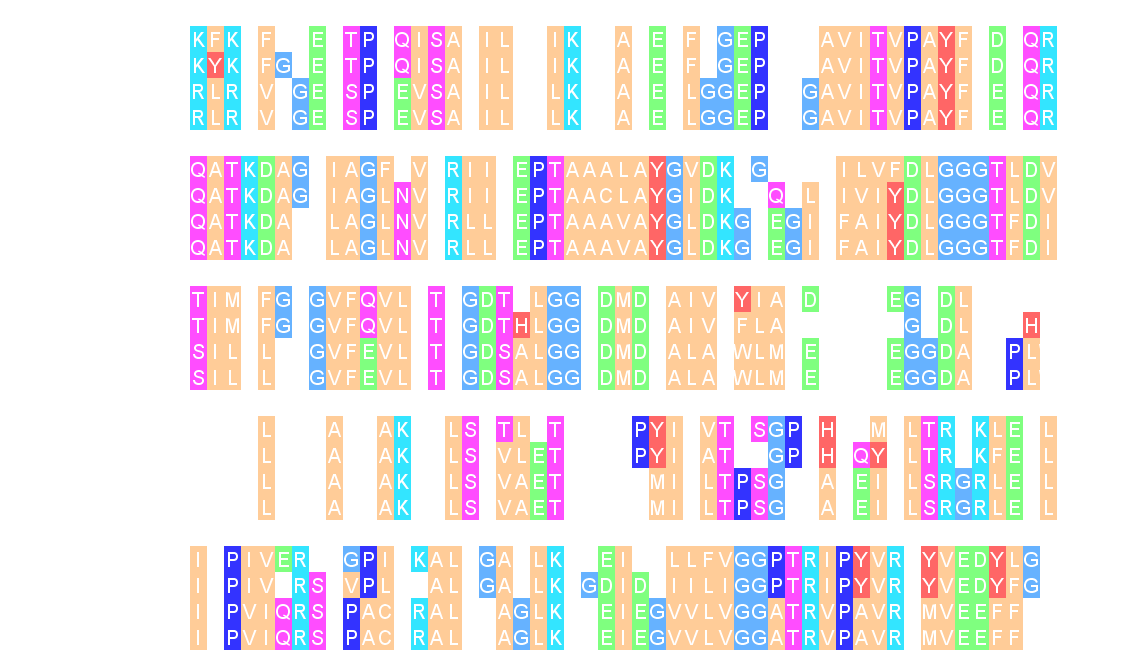
\includegraphics[height=0.9\textheight]{alighment}

\end{frame}


\section{Общие рассуждения}
\begin{frame}{Как устроено вещество?}
   \begin{itemize}
     \item Первые шаги к пониманию того, что вещество состоит из маленьких элементов сделал Лукреций, давно. 
    \vspace{0.2cm}
     \item Первые эксперименты по установлению структуры  были проведены только в начале 20 века
    \vspace{0.2cm}
     \item Появились специальные молекулярные наборы из шариков и палочек
    \vspace{0.2cm}
     \item Правильное использование химической информации позволило строить первые модели,
         очень похожие на результаты РСА.
    \end{itemize}
\end{frame}

\begin{frame}{Как это работает?}
    \centering
    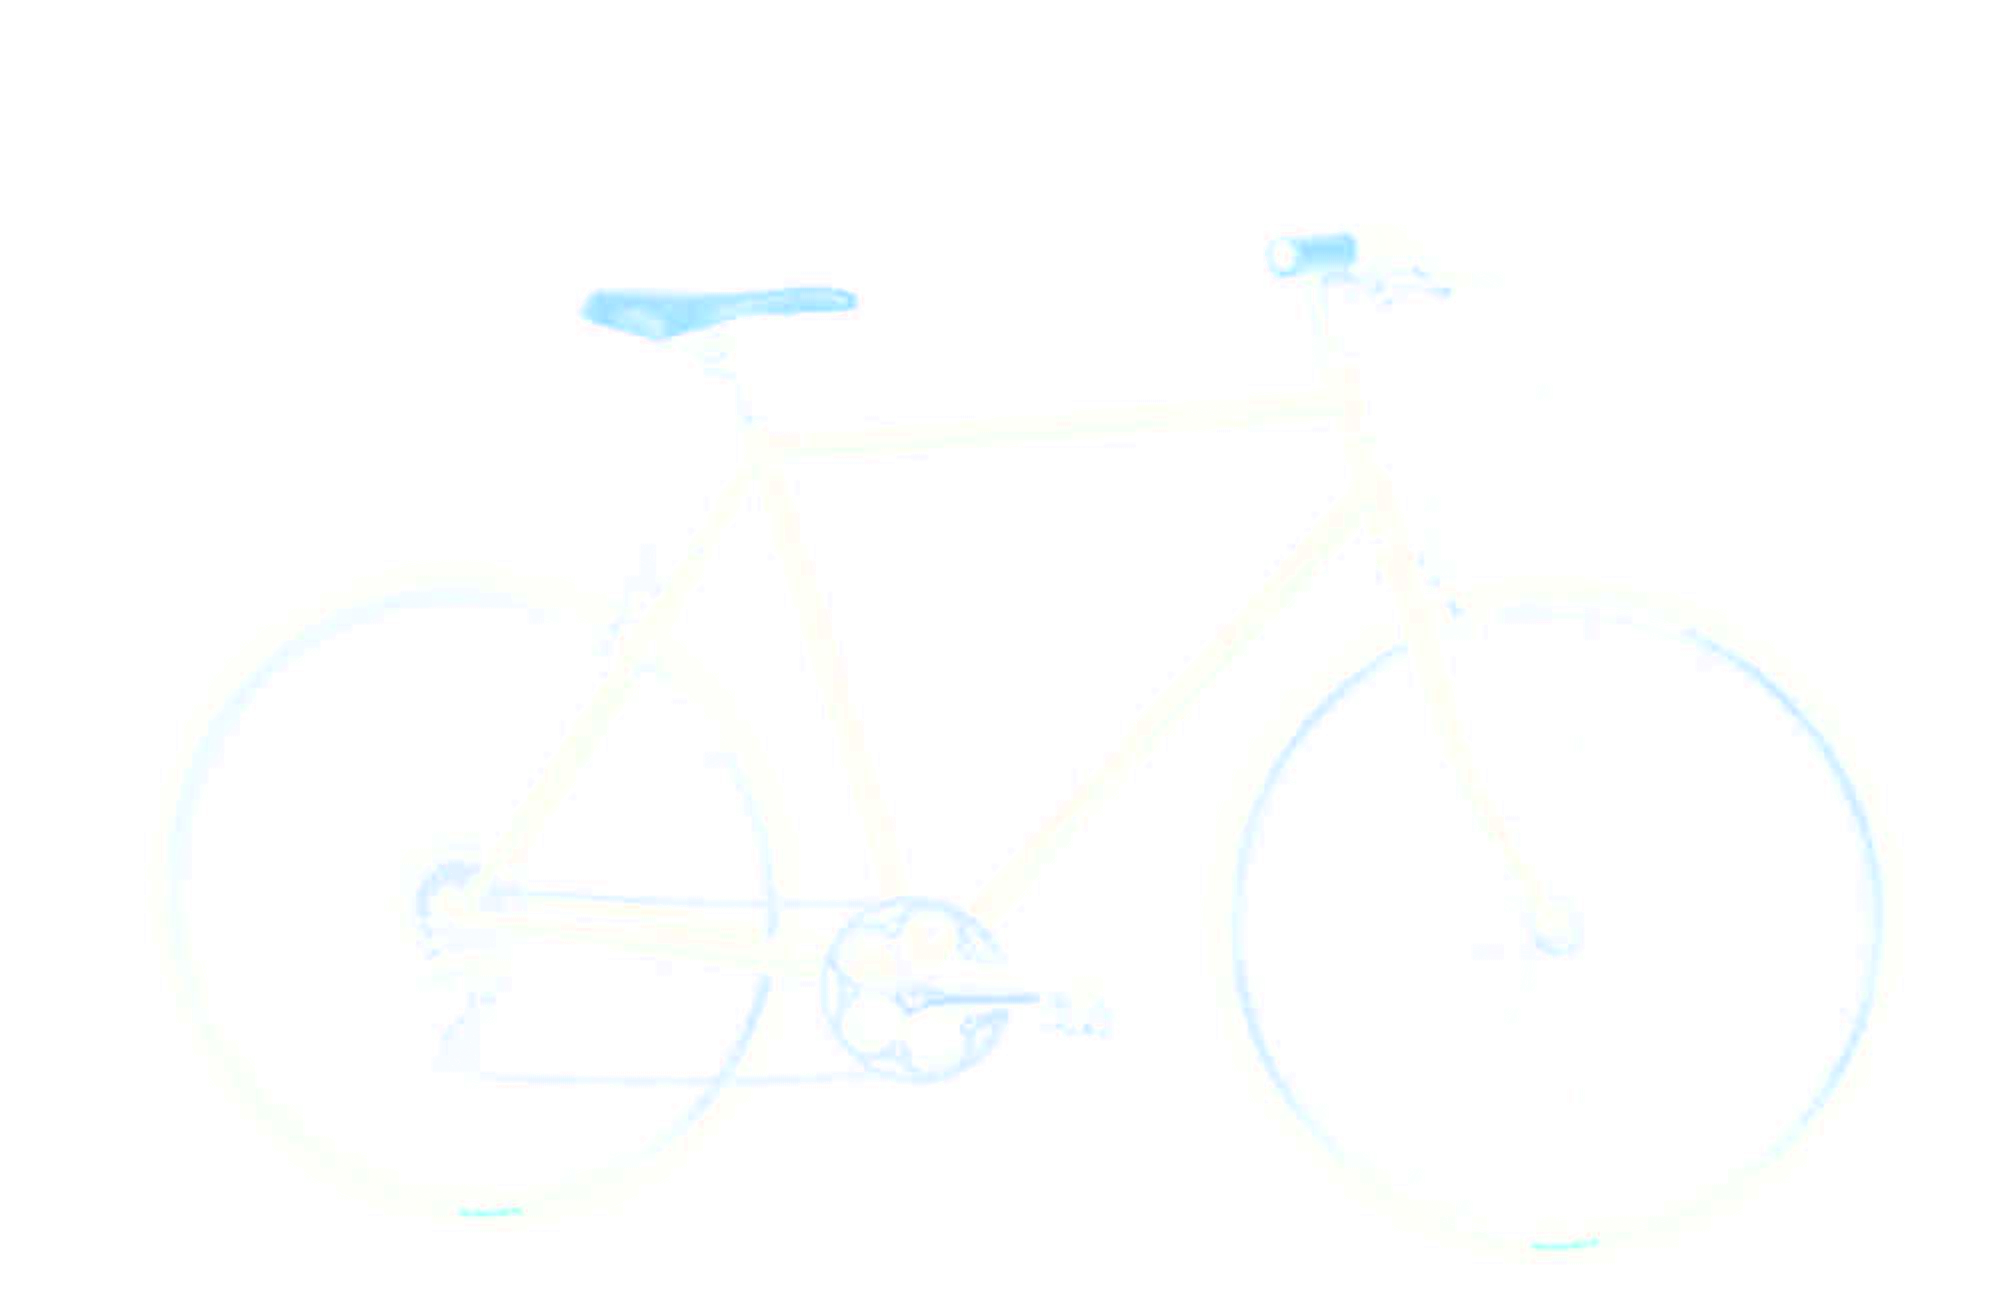
\includegraphics[height=0.9\textheight]{bicycle}
\end{frame}

\begin{frame}{Для чего нужны модели?}
  \begin{itemize}
   \item
Упрощение сложного объекта до анализа только той части которая предполагаемо является объектом интереса.\\
    \vspace{0.5cm}
   \item
Модель является иллюстрацией для дедуктивного анализа очень сложных или многочисленных явлений.\\
    \vspace{0.5cm}
   \item
Часто модели отражают  реальность не полностью, но моделируемой точности бывает достаточно для понимания рассматриваемой системы.
\end{itemize}
\end{frame}


\begin{frame}{Финальный этап: Дизайн}
    Моделирование структуры, определение свойств это шаги к самому важному этапу : \\
    \vspace{0.5cm}
    \textbf{
    дизайну или проектированию нового с заданными свойствами.}
\end{frame}

\begin{frame}{Маcштабы в моделировании}
    %      \includegraphics[width=0.9\textwidth]{scope}
    \centering
    \begin{tikzpicture}[every node/.style={scale=0.9}]
    \begin{axis}
        [
        ,width=0.8\textwidth
        ,height=0.8\textheight
        ,xlabel={Размер}
        ,ylabel={Время}
        %,xtick=data,
        ,xtick={0,1,...,4}
        ,xticklabels={'',A,нм,мкм,мм,м}
        ,yticklabels={'',фс,пс,нс,мкс,мс,с,часы, годы}
        ]
        %\addplot+[sharp plot] coordinates   {(0,18.26) (1,21.47) (2,24.58) (3,24.95)};
    \end{axis}
    \draw[draw=black,fill=red!10!black] (0,0) rectangle ++(2.5,1) node[pos=.5] {Электроны};
    \draw[draw=black,fill=yellow!10!black] (1.5,0.8) rectangle ++(2.5,1) node[pos=.5] {Атомы};
    \draw[draw=black,fill=green!10!black] (3,1.6) rectangle ++(3,2) node[pos=.5] {Группы атомов};
    \draw[draw=black,fill=blue!10!black] (5.5,3.4) rectangle ++(4,3) node[pos=.5] {Cплошные среды};
%\draw (0,0) rectangle (2,1) node[pos=.5] {КМ};
%\draw (1.5,1) rectangle (2,1) node[pos=.5] {MМ};
\end{tikzpicture}
\end{frame}

\begin{frame}{Компьютер}
    \begin{itemize}
     \item Формально для решения задач моделирования компьютер не является обязательным элементом
    \vspace{0.2cm}
     \item Быстрый компьютер значительно увеличивает точность и широту исследования, и следовательно достоверность моделирования.
    \vspace{0.2cm}
     \item Количество вычислений отражает степень исследования конформационного
         пространства
    \end{itemize}
\end{frame}

\begin{frame}{Компьютер и программы}
    Those programs \textbf{always provide a result}, the evaluation of which is at liberty of the user. The programs 
    \textbf{tend stubbornly} to calculate \textbf{every absurd application} and present a result-not only a number, but also a graph and
    represent a further instrument of seduction for the uncritical use of algorithms. 
\end{frame}





	


